\section{Introducción}
\noindent El objetivo de esta práctica es el estudio del comportamiento de diferentes disoluciones amortiguadoras (también llamadas disolución tampón) mediante varias medidas del pH. También se realizará una valoración potenciométrica (es decir, basada en la diferencia de potencial a través de un electrodo) con \ce{H3PO4}.
\section{Inventario}
\vspace{0.4cm}
Para esta práctica hemos usado:

\begin{multicols}{2}
    \begin{itemize}
        \item 1 Peachímetro
        \item 2 Pipetas graduadas
        \item 3 Propipetas
        \item 1 Colador
        \item 1 Varilla metálica
        \item 1 Placa de calor
        \item 2 Frascos lavadores
        \item 4 Vasos de precipitados
        \item 1 Embudo
        \item 3 Erlenmeyer
        \item 2 Espátulas
        \item 2 Probetas
        \item Líquidos: 
        \item Naranja de metilo ($\ce{C14H14N3NaO3S}$)
        \item Fenolftaleína ($\ce{C20H14O4}$)
        \item Agua ($\ce{H2O}$)
    \end{itemize}
\end{multicols}

\vspace{0.3cm}
Podemos ver parte de lo nombrado anteriormente en la siguiente fotografía:

\begin{figure}[H]
    \centering
    \hspace*{-2.3cm}
        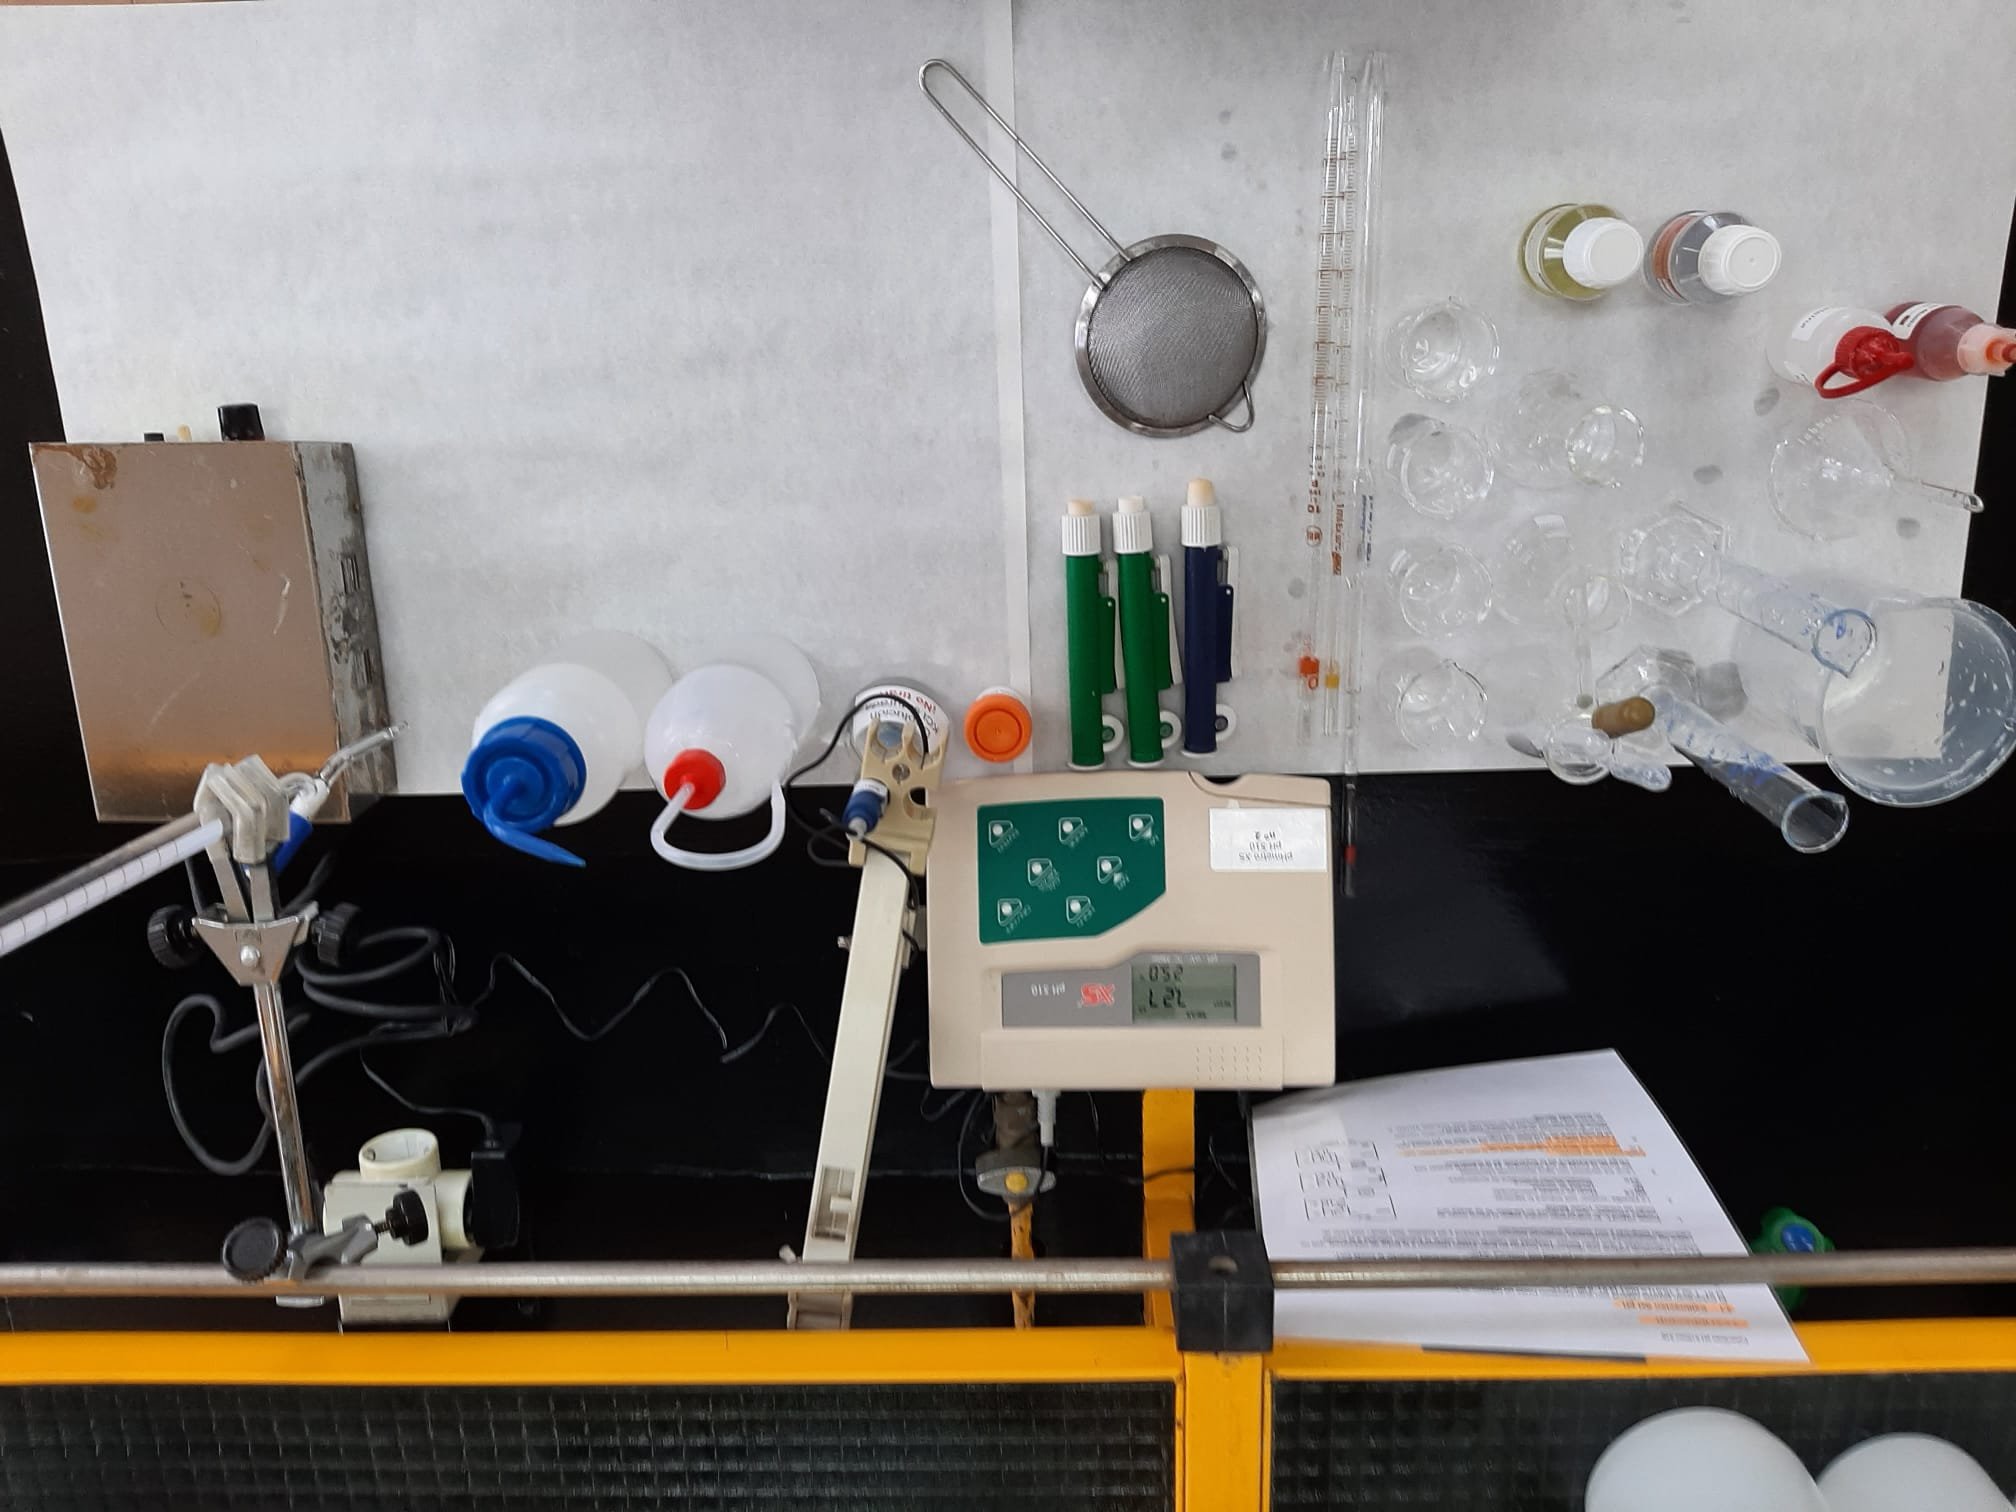
\includegraphics[scale = 0.15, angle=180]{prac3/Inventario3.jpeg}
    \hspace*{-2.3cm}
    \vspace{-2cm}
\end{figure}

\clearpage

\section{Procedimiento}
\noindent En primer lugar, mediremos el pH de ciertas disoluciones amortiguadoras, de la cual siempre tendremos $V_{disolución} = 30 \si{ml}$ a los cuales añadiremos $10 \si{ml}$ primero de una base fuerte (\ce{NaOH} 1\si{M}) y luego de un ácido fuerte (\ce{HCl} 1\si{M}). Posteriormente, repetiremos la adición de esta base y este ácido, ahora añadiéndolos a 30 \si{ml} de agua destilada.\\\\
Para la valoración potenciométrica, añadiremos unas gotas de naranja de metilo y de fenolftaleína a 10 \si{ml} de \ce{H3PO4}. Ahora, añadiremos \ce{NaOH} hasta que se vuelva amarillo desde su color rosa inicial para luego seguir añadiendo hasta que vuelva a dicho rosa. Esta experiencia la repetiremos tres veces para poder comparar las medidas de volumen obtenidas.\\\\
Finalmente, repetiremos el paso anterior pero ahora de forma mucho más precisa: con ayuda de la varilla imantada y del pH-metro, añadiremos \ce{NaOH} de 2 \si{ml} en 2 \si{ml}, excepto cerca del volumen de viraje, donde añadimos de 0,2 en 0,2 \si{ml}, e iremos midiendo los cambios de pH en estos intervalos.

\clearpage
\section{Cuestiones}
\noindent\textcolor{BlueViolet}{\textbf{\textit{a) Busque en el Handbook el valor de $K_a$ para el ácido acético.}}}\\\\
\noindent El valor de $K_a$ que encontramos en el \textquote{\textit{CRC Handbook of Chemistry and Physics}} es de $K_a = 1.75\cdot 10^{-5}$ a $25^{\circ} C$\\\\
\noindent\textcolor{BlueViolet}{\textbf{\textit{b) Comente si:
    \begin{itemize}
        \item El $pH$ de la disolución tampón es función de la concentración.
        \item La capacidad amortiguadora depende de la concentración de la disolución tampón.
        \item Coinciden los valores de $pH$ esperados teóricamente con los medidos experimentalmente. Comente las posibles fuentes de error.
    \end{itemize}
}}}

\noindent Para esta primera parte de la cuestión podemos afirmar que el pH de cualquier disolución tampón es proporcional directamente a su concentración. En concreto a la relación entre la concentración de sal y de ácido que nos dice la ecuación de Henderson-Hasselbalch:
\[pH = pK_a + \log\left(\frac{[S]}{[A]}\right)\]
\noindent En segundo lugar, estudiaremos si la capacidad amortiguadora de la disolución tampón depende también de la concentración. Y efectivamente, lo hace, puesto que depende no solo de la concentración de la disolución, sino de la concentración de todo el sistema, aumentando junto con ella, alcanzando el máximo cuando el cociente se aproxima a 1.\\\\
\noindent Por último, comprobaremos si los valores del ph experimentales coinciden con los esperados teóricamente. Para el caso de viraje de rosado a amarillo, de forma teórica vemos que deberíamos notar el cambio alrededor de los $11 ± 0.5 \si{ml}$, pero experimentalmente la notamos en $10.4 ± 0.2 \si{ml}$. De igual manera ocurre en el cambio de vuelta de amarillo a rosa. Debería cambiar sobre de los $22 ± 0.5 \si{ml}$ pero lo hace entorno a los $21.4 ± 0.2 \si{ml}$.\\\\
\noindent La mayor parte de este error se debe claramente al factor humano. Nuestra primera valoración es potenciométrica, tratamos de dilucidar en qué instante la disolución lleva a cabo este viraje de color, pero introducimos una gran cantidad de error al no ser un punto claro el que produce este viraje.
\clearpage

\noindent Vamos a representar en una gráfica la tabla de ph frente al volumen de \ce{NaOH} añadido. La tabla que describe los datos está representada en la hoja 21.

\begin{figure}[H]
    \centering
    \hspace*{-2.3cm}
        \includegraphics[scale = 1]{prac3/Gráfica3).jpg}
    \hspace*{-2.3cm}
    \caption{Ph frente al volumen añadido}
\end{figure}

\noindent Se puede observar en la gráfica un ajuste polinomial de grado 6 que aproxima nuestros datos. Se aprecian a la perfección los dos cambios del pH, así como el ascenso final que se sale de nuestros datos.\\\\
\noindent A continuación, representaremos la curva derivada de esta mediante el cociente incremental para poder ver más claramente cuales son nuestros puntos de viraje. Para ello, añadimos a nuestra tabla de datos de ph y volúmen, los apartados que se basan en las siguientes expresiones:

\[\frac{V_{i+1}+V_i}{2}\]
\[\frac{pH_{i+1}-pH_i}{V_{i+1}-V_i}\]
\clearpage

\begin{figure}[H]
    \centering
    \hspace*{-2.3cm}
        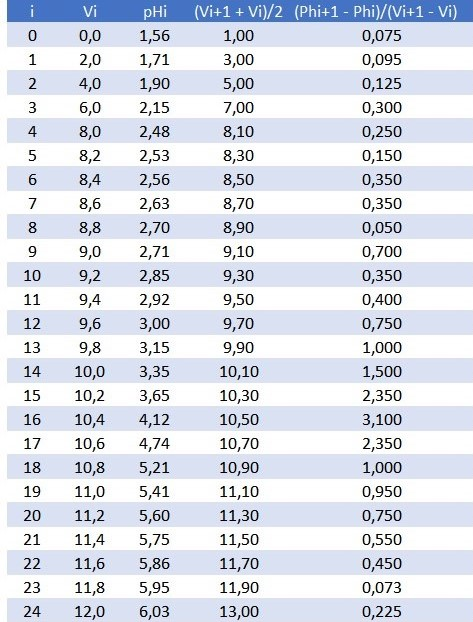
\includegraphics[scale = 0.75]{prac3/tabla31.jpg}
        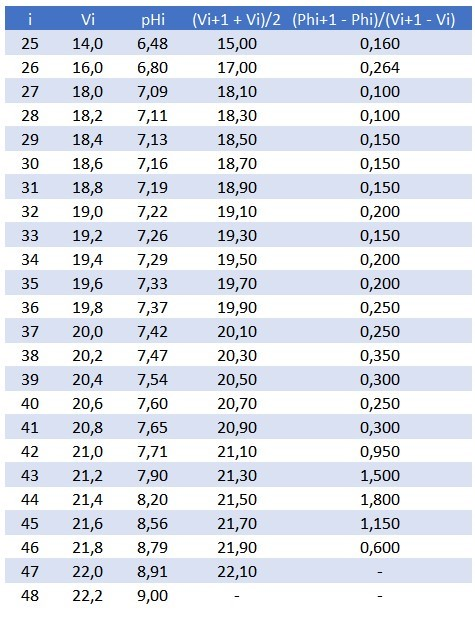
\includegraphics[scale = 0.75]{prac3/tabla32.jpg}
    \hspace*{-2.3cm}
\end{figure}

\noindent Una vez obtenidos los datos, representamos gráficamente la derivada de la gráfica anterior, que resulta muy interesante por la aparición de dos picos explícitos allá donde el pH ha variado muy velozmente.

\begin{figure}[H]
    \centering
    \hspace*{-2.3cm}
        \includegraphics[scale = 0.8]{prac3/Gráfica3.1.jpg}
    \hspace*{-2.3cm}
\end{figure}
\clearpage

\noindent En esta gráfica, podemos observar que los máximos se encuentran en los puntos 10.4 y 22.5 siendo el primero más pronunciado que el segundo. Estos valores coinciden con lo observado experimentalmente.\\\\
\noindent Por último, calcularemos la concentración inicial de ácido fosfórico - \ce{H3PO4} – a partir de estos volúmenes. Si sabemos los volúmenes de viraje, podemos plantear la ecuación que rige esta reacción para ver la relación molar entre \ce{H3PO4} y \ce{NaOH}. Como sabemos la concentración de la disolución de \ce{NaOH}, podremos calcular los moles de \ce{H3PO4}, y con ellos el valor pedido.\\\\
\noindent La reacción se desarrolla de la siguiente forma:
\[\ce{H3PO4 + NaOH -> H2PO2^- + Na^+ + H2O}\]
Con la reacción ajustada, comprobamos que a cada mol de \ce{NaOH} le corresponde un mol de ácido fosfórico. Haremos entonces el siguiente cambio de conversión para obtener los moles de ácido, tomando como volumen de \ce{NaOH} el primer volumen de viraje:
\[10.3\si{ml}\ \text{de}\ \ce{NaOH}\cdot\frac{1\si{L}}{1000\si{ml}}\cdot \frac{1\si{mol}\ \ce{NaOH}}{1\si{L}\ \text{disolución}\ \ce{NaOH}}\cdot\frac{1\si{mol}\ \ce{H3PO4}}{1\si{mol}\ \ce{NaOH}} = 0.0103\si{mol}\ \ce{H3PO4}\]
Ahora obtenemos la molaridad:
\[M_{\ce{H3PO4}} = \frac{n_{\ce{H3PO4}}}{L_{\ce{H3PO4}}} = \frac{0.0103}{0.01} = 1.03\si{M}\]
\noindent Probablemente gran parte del error se debe a la búsqueda de colores más intensos de lo debido a la hora de realizar la valoración potenciométrica. Esto ha hecho que la disolución avance más de lo debido en la valoración, haciendo que su pH aumente excesivamente antes de tomar los volúmenes de \ce{NaOH} que supusimos serían de viraje.\\\\
\noindent En lo respectivo a las gráficas realizadas en la tercera cuestión, ambas representan de forma muy fidedigna los cambios de pH sufridos por la disolución. En la primera, podemos ver de forma directa el crecimiento del pH conforme aumentamos el volumen de la base. 
\noindent Mientras estemos alejados de los puntos de viraje, destacamos como el crecimiento es muy cercano a un crecimiento lineal. Sin embargo, en estos puntos críticos nombrados, el crecimiento se vuelve prácticamente exponencial.\\\\
\noindent Esto queda reflejado muy claramente en la segunda gráfica, la de la derivada, que mantiene valores constantes hasta llegar a máximos muy pronunciados, en especial el primero, que muestran estos puntos de viraje muy bruscos. Concluimos que ambas gráficas concuerdan con los resultados experimentales y teóricos, en el sentido de representar cambios bruscos en el color de la disolución.